\section{Source reconstruction}

\begin{figure}
\centering 
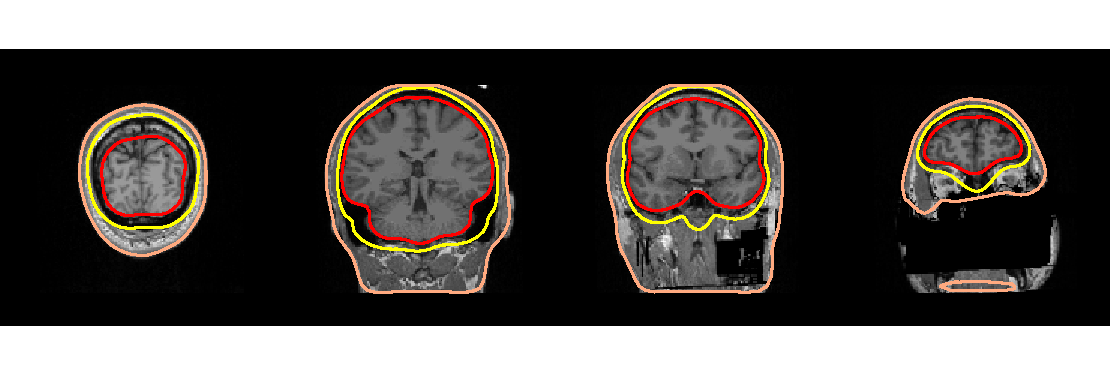
\includegraphics[width=\linewidth]{figures/sub001_bem.pdf}
\caption[BEM surfaces on flash MRI images.]{BEM surfaces on flash MRI images. The inner skull, outer skull and outer skin are outlined in color.}
\label{fig:fig_bem}
\end{figure}

The MNE software relies on the FreeSurfer package~\citep{dale-fischl-etal:99,fischl-serena-etal:99} for the processing of anatomical MRI images. This automatic procedure is run using the command \code{recon-all} on the T1 MRI of each subject. This provides many useful pieces of information, but the most critical here are the cortical reconstruction (a high resolution triangulation of the interface between the white and the gray matter) and the inner skull surface.

For inverse source reconstruction and beamforming, we must first compute the forward solution, often called a gain or lead field matrix. It describes the sensitivity of the sensors to a given set of dipoles~\citep{mosher-leahy-etal:99}. Computing the gain matrix, which is a linear operator, requires having a so-called source space of dipole locations, a conductor model for the head, and the sensor locations relative to those dipoles. This latter requirement in practice means putting in the same coordinate system the MRI (where the source space and conductor model are defined), the head (where the EEG electrodes are digitized), and the MEG device (where the MEG sensors are defined). This step is commonly referred to as \emph{coregistration}. We will cover each of these steps below.

\subsection{Source space}
As we expect most of our activations of interest to be due to cortical currents~\citep{dspm}, we position the candidate dipoles on the cortical mantel. We chose a source space obtained by recursively subdividing the faces of an octahedron six times (oct6) for both the left and right hemispheres. This leads, for each subject, to a total of 8196 dipoles evenly spaced on the cortical surface (See Figure 6 in \citep{mne}).

\subsection{Head conductivity model}
MNE can use simple spherical conductor models but when the MRI of subjects are available, the recommended approach is to use a piecewise-constant conductivity model of the head. Tissue conductivities are defined for each region inside and between the segmented interfaces forming the inner skull, outer skull and the outer skin. It corresponds to a so-called three layer model, however a single layer is possible when using only MEG data. The default electrical conductivities used by MNE are 0.3 S/m for the brain and the scalp, and 0.006 S/m for the skull, i.e., the conductivity of the skull is assumed to be 1/50 of that of the brain and the scalp. With such a head model, Maxwell equations are solved with a \ac{BEM}.

In addition to the T1 MRI image, \ac{FLASH} images are provided in the present dataset. Such MRI images allow to automatically extract precise surfaces for the inner skull and outer skull. Note that in the absence of FLASH images, MNE offers a somewhat less accurate solution based on the watershed algorithm. One output of the MNE automatic BEM surface extraction is presented in Figure~\ref{fig:fig_bem}. It contains the three surfaces needed for the computation of the EEG gain matrix. In our results shown here, we used only the MEG data for source reconstruction, and consequently only made use of the inner skull surface in a one-layer model. As MRIs shared here are defaced, outer skull and scalp surfaces are anyway quite wrong, so we considered it satisfactory to only use the inner skull surface.

Quality insurance at this stage consists in checking that the three surfaces do not intersect with each other and that they follow the interfaces between the brain, the skull and the skin. A slice-by-slice visual inspection of approximate alignment is best and is conveniently proposed by MNE BEM plotting function that outputs a figure as presented in Figure~\ref{fig:fig_bem}.

Here, as the MRIs shared in this dataset were anonymized, the outer skin surface obtained automatically using Freesurfer intersected with the outer skull surface for most subjects. However this is  rarely observed with non defaced T1 MRI images.

\subsection{Coregistration}
In order to compute the gain matrix, the sensor locations (and normals), head model, and source space must be defined in the same coordinate system. In practice, this means that the BEM surfaces and source space (which are defined in MRI coordinates) must be coregistered with the EEG sensors, which are digitized in the Neuromag head coordinate frame (defined by the digitized nasion, LPA, and RPA). The MEG sensor locations and normals are defined in the MEG device coordinate frame. Typically, the MEG-to-head transformation is determined during acquisition using head position indicator (HPI) coils (or redefined using head position transformation using Maxwell filtering), so MEG sensors can be easily transformed to head coordinates. The transformation between the MRI and head coordinate frames is typically estimated by identifying corresponding points in the head and MRI coordinate systems, and then aligning them.

The most common points used to provide an initial alignment are the fiducial landmarks that define the Neuromag head coordinate frame. They consist of the nasion and two pre-auricular points which are digitized during acquisition, and are then also identified by offline visual inspection on the MRI images. Additional digitization points on the head surface can also be used to better adjust the coregistration. In this study, on average, 135 digitization points were available per subject. The transformation, which consists of a rotation matrix and a translation vector, is then typically saved to a small file, also called \emph{trans} file, and later used to compute the forward solution.

For quality insurance, MNE offers a simple function to visualize the result of the coregistration.
Figure~\ref{fig:fig_trans} shows one example obtained with this function with the defaced, low-resolution MRI head surface. As here the MRI were defaced, many important digitization points close to the nose where useless. To reduce the risk of bad coregistration due to defaced MRI images, we used the trans files kindly provided by the original authors.
    
\begin{figure}
\centering
    
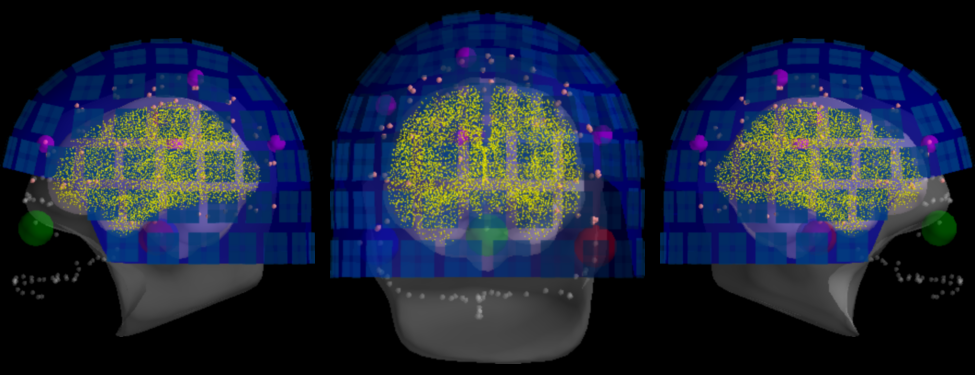
\includegraphics[width=\linewidth]{figures/sub001_alignment.pdf}
 \caption[Visualization of coregistration quality]{The result of head-to-MRI (and MEG-to-head) transformations with inner skull and outer skin surfaces for one subject. Note that the MEG helmet is well-aligned with the digitization points. The digitized fiducial points are shown with large dots, EEG electrodes with small pink dots, and extra head digitization points with small gray dots. Note that the anonymization of the MRI produces a mismatch between digitized points and outer skin surface at the front of the head.}
\label{fig:fig_trans}
\end{figure}

\subsection{Covariance estimation and Whitening}

As inverse solvers typically assume Gaussian noise distribution on the sensors with an identity covariance matrix, a whitening step is first necessary~\citep{engemann2015automated}. M/EEG signals are indeed highly spatially correlated. Whitening also allows integration of data from different channel types that can have different units and signal amplitudes which differ by orders of magnitudes (cf. planar gradiometers, axial magnetometers, and EEG electrodes).
To whiten the data, one must provide an estimate of the spatial noise covariance matrix. This can be computed from empty-room recordings for MEG or pre-stimulus periods~\citep{mne}. Here, we followed the approach proposed by~\citet{engemann2015automated}, which consists in picking the best model and estimating the best regularization parameters by computing the Gaussian log-likelihood of left-out data (i.e., a cross-validation procedure). Such an approach has been shown to be particularly robust for scenarios where a limited number of samples is available for covariance estimation.

In this analysis, the noise covariance is estimated from the 200\,ms of data before stimulus presentation. During this period, only a fixation color is visible at the center of the screen. Given this covariance matrix and the gain matrix, one can assemble the inverse operator to compute the MNE or dSPM solutions~\citep{dspm}.

The quality of the covariance estimation and whitening can have a significant impact on the source localization results. The rank-adjusted global field power (GFP) has been proposed by \citet{engemann2015automated} as a measure that can be used to check the quality of the whitening. It is defined as GFP$=\sum_i x^2_{i} / P$ where $P$ is the rank of the data and $x_i$ is the signal in the $i$th sensor at a time instant. The GFP being a normalized sum of Gaussian random variables with an identity covariance matrix, it follows a $\chi^2$ distribution with an expected value of 1. What is not captured by our noise model, e.g. actual brain signals, thereof will pop out in the whitened domain.
To understand this better, we show some whitened data and the GFP in Figure~\ref{fig:plot_white}. If the Gaussian assumption has not been violated, we expect the whitened data to contain 95\% of the signal within the range of -1.96 and 1.96, which we mark in dotted red lines. The baseline period, where we estimated our noise covariance from, appears to satisfy this assumption. Consequently, the GFP is also 1 during this period. One can observe a strong increase in the GFP just after the stimulus onset, and that it returns slowly to 1 at the end of the time interval. Such a diagnostic plot can in fact be considered essential for quality assurance before computing source estimates. This has as consequence that what appears in the source estimates depends on our noise model. For instance, using a noise covariance obtained from empty room recordings would suggest the presence of ``interesting'' signals, simply because it contains brain signals that are fundamentally different from the empty room noise.

For the LCMV beamformer, we also need to estimate a signal covariance. For this we use the 30\,ms to 300\,ms window after the stimulus onset. The data covariance is again regularized automatically following~\citep{engemann2015automated} and is motivated by the results from~\citep{Woolrich:2011,MindTheCov}.

\begin{figure}
\centering
 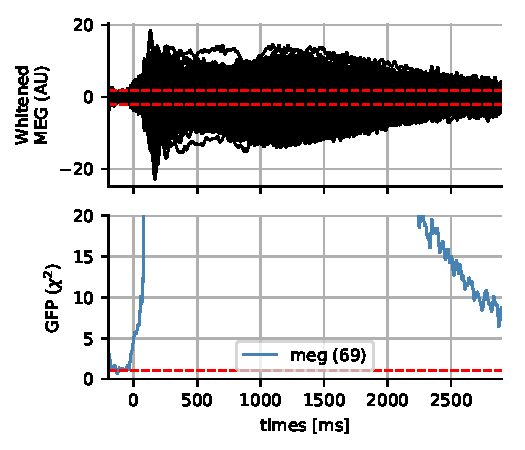
\includegraphics{figures/sub004_highpass-NoneHz-plot_white_meg.pdf}
\caption[Whitened MEG data at the evoked level for one subject]{Whitened MEG data for subject 4 and the global field power (GFP) which follows a $\chi^2$ distribution if the data is assumed Gaussian. The dotted horizontal red lines represent the expected GFP during the baseline for Gaussian data. Here the data slowly return to baseline at the end of the epoch.}
\label{fig:plot_white}
\end{figure}

\emph{Caveats.} If empty-room data are used to whiten processed signals, one must make sure that the obtained noise covariance matrix corresponds to the processed data rather than to the original empty-room data. This is done by processing the empty-room data with exactly the same algorithm and the same parameters as the actual data to be analyzed. For example if SSS, SSP or ICA are applied on processed data, it should be applied to empty room data before estimating the noise covariance. Concretely, SSP vectors and ICA components projected out from the data of interest should also be projected out from the empty room data. SSS should be performed with identical parameters.
Also note that magnetometers and gradiometers are whitened jointly. Moreover, if SSS was applied, the display of whitening treats magnetometers and gradiometers as one channel-type. For proper assessment of whitening, a correct assessment of the spatial degrees of freedom is necessary. The number of SSS dimensions is commonly a good estimate for the degrees of freedom. When movement compensation was applied, the estimated data rank maybe unreliable and suggest too many independent dimensions in the data. Even the actual number of SSS components can be misleading in such circumstances. It is then advisable to inspect the eigenvalue spectrum of the covariance matrix manually and specify the degrees of freedom manually using the rank parameter.

\subsection{Inverse solvers and beamforming}
% Given the gain matrix $\mathbf{G}$, our data can be expressed as:
% \begin{equation}
% \mathbf{M} = \mathbf{GX} + \mathcal{P}(\mathbf{X)}
% \end{equation}
% where $\mathbf{M}$ is the sensor-space data, $\mathbf{G}$ is the gain matrix and $\mathbf{X}$ is the source time course. Often, a penalty term $\mathcal{P}(\mathbf{X)}$ is also applied to inject certain constraints on the data, such as sparsity or smoothness.

The goal of an inverse solver is to estimate the locations and the time courses of the sources that have produced the data. While the data $\mathbf{M}$ can be expressed linearly from the sources $\mathbf{X}$ given the gain matrix $\mathbf{G}$, $\mathbf{M} \approx \mathbf{GX}$, the problem is ill-posed. Indeed $\mathbf{G}$ has many more columns than rows. This means that there are more unknown variables (brain sources) than the number of measured values (M/EEG sensors) at each time point. This also implies that the solution of the inverse problem is not unique.

For this reason, many inverse solvers have been proposed in the past ranging from dipole fits~\citep{scherg-etal:85,mosher-lewis-etal92}, minimum norm estimates (MNE)~\citep{Hamalainen:1984}, and scanning methods such as RAP-MUSIC or beamformers such as LCMV and DICS \citep{Van_Veen:1997,gross-etal:2001,Sekihara:2005}. There is therefore no absolute perfect inverse solver, although some are more adapted than others depending on the data. Some are adapted to evoked data for which one can assume a few set of focal sources. Some also give you source amplitudes in a proper unit, which is nAm for electrical current dipoles, such as MNE, MxNE~\cite{gramfort-etal:2013} or dipole fits. Some give you spatially normalized statistical maps such as dSPM~\citep{dale2000dspm} or LCMV combined with neural activation index (NAI) filter normalization~\citep{Van_Veen:1997}.

Given the important usage of dSPM and the LCMV beamformer in the cognitive neuroscience literature, we wanted to investigate how much using one of these two most commonly used methods was affecting the source localization results. The dSPM solution was computed with MNE default values: loose orientation of 0.2, depth weighting~\citep{lin2006assessing} of 0.8, and SNR value of 3. The LCMV used was a vector beamformer with unit-noise-gain normalization~\citep{Sekihara:2005} as implemented in MNE 0.15. No specific regularization was used in the beamformer filter estimation.

% \subsubsection{Dynamic Statistical Parameter Mapping (dSPM)}

% dSPM~\citep{dale2000dspm} is similar to Minimum Norm Estimates (MNE) but produces a statistical map of where the activity is different from background noise. In that sense, the dSPM source activations do not have a physical unit. The consequence of this normalization is that it removes the bias towards superficial sources that is present in MNE. The inverse solver produces a spatiotemporal estimate but in Figure~\ref{fig:fig_stc}, we visualize the spatial activations in only a single time point of interest. The source estimates are visualized by smoothing the data to fit the vertices in the tessellation of the cortical surface (Figure~\ref{fig:fig_stc}). In MNE, \emph{smoothing} is an iterative process which blurs the data to the surface.
 
% \subsubsection{Linearly Constrained Minimum Variance (LCMV) beamforming}

% LCMV is a spatial filter used to estimate the sources. The filter works by passing the activity at a certain location while attenuating the noise from other locations. It requires only that the sources are uncorrelated. It tends to give more focal activation maps compared to conventional source localization methods~\citep{vanveen-etal:1997}. This is what we observe also in our experiments in Figure~\ref{fig:fig_stc}.

% It is however not always clear if the sources are correlated or not. If they are, LCMV results can lead to large errors in the source estimates \citep{vanveen-etal:1997,hansen2010meg}.